% !TeX TXS-program:compile = txs:///xelatex/[--shell-escape]
\documentclass[11pt, a4paper, nofootinbib]{article}

\usepackage{fontspec}
\usepackage{textcomp, gensymb}
\usepackage[australian]{babel}
\usepackage{alphabeta}
\usepackage{microtype}
\usepackage[table,xcdraw]{xcolor}
\usepackage{colortbl}
\usepackage[top=12mm, bottom=10mm, left=12mm, right=12mm, headsep=4mm, footskip=8mm]{geometry}
\usepackage{array}
\usepackage[export]{adjustbox}
\usepackage{datetime}
\usepackage{graphicx}
\usepackage{svg}
\usepackage{float}
\usepackage{subcaption}
\usepackage{caption}
\usepackage{tikz}
\usepackage{relsize}
\usepackage{circuitikz}
\usepackage{pgfplots}
\pgfplotsset{compat=newest}
\usepackage{cuted}
\usepackage{titletoc}
\usepackage[showboxes, absolute]{textpos}
\usepackage{booktabs}
\usepackage{multicol}
\usepackage{longtable}
\usepackage{multirow}
\usepackage{tabularx}
\usepackage{tabularray}
\usepackage[thinlines]{easytable}
\usepackage{amsmath}
\usepackage[official]{eurosym}
\usepackage{enumitem}
\usepackage[style=apa, backend=biber, hyperref=true, natbib=true, uniquename=full, maxcitenames=999, mincitenames=999, sortcites=true, sorting=apa]{biblatex}
\addbibresource{refs.bib}
\usepackage{nameref}
\usepackage[
  hidelinks,
  colorlinks=true,
  linkcolor=black,
  urlcolor=black,
  filecolor=black,
  citecolor=blue,
  linktoc=all
]{hyperref}
\usepackage[capitalise,nameinlink,noabbrev]{cleveref}
\usepackage{ragged2e}
\usepackage{listings}
\usepackage[bottom]{footmisc}
\usepackage{paracol}
\usepackage{stfloats}
\usepackage{xurl}
\usepackage{eso-pic}
\usepackage{titlesec}
\usepackage[]{appendix}
\usepackage{fancyhdr}
\usepackage{changepage}

\crefname{appsec}{appendix section}{appendix sections}
\Crefname{appsec}{Appendix Section}{Appendix Sections}

\crefname{appendix}{appendix section}{appendix sections}
\Crefname{appendix}{Appendix Section}{Appendix Sections}

\usepackage{etoolbox}
\BeforeBeginEnvironment{appendices}{%
  \clearpage
  \appendix
  \crefalias{section}{appendix}%
  \crefalias{subsection}{appendix}%
  \crefalias{subsubsection}{appendix}%
  \crefalias{subsubsubsection}{appendix}%
}


\setmainfont{Inter}[
    Path = ./font/,
    UprightFont = {Inter_28pt-Regular.ttf},
    BoldFont = {Inter_28pt-Bold.ttf},
    ItalicFont = {Inter_28pt-Italic.ttf},
    BoldItalicFont = {Inter_28pt-BoldItalic.ttf}
]

\linespread{1.15}
\setlength{\parskip}{8pt plus 2pt minus 2pt}
\setcounter{tocdepth}{4}
\setcounter{secnumdepth}{4}
\widowpenalty=10000
\clubpenalty=10000

\definecolor{SectionBGColor}{HTML}{0066ff}

\titleclass{\subsubsubsection}{straight}[\subsubsection]
\newcounter{subsubsubsection}[subsubsection]
\renewcommand{\thesubsubsubsection}{\thesubsubsection.\arabic{subsubsubsection}}

\titleformat{\section}{\normalfont\Large\bfseries\color{SectionBGColor}}{\thesection}{1em}{}
\titleformat{\subsection}{\RaggedRight\normalfont\large\bfseries\color{SectionBGColor}}{\thesubsection}{1em}{}
\titleformat{\subsubsection}{\normalfont\normalsize\bfseries\color{SectionBGColor}}{\thesubsubsection}{1em}{}
\titleformat{\subsubsubsection}{\normalfont\normalsize\bfseries\color{SectionBGColor}}{\thesubsubsubsection}{1em}{}
\titleformat{\paragraph}[runin]{\normalfont\normalsize\bfseries\color{SectionBGColor}}{\theparagraph}{1em}{}

\titlespacing*{\section}{0pt}{6pt}{2pt}
\titlespacing*{\subsection}{0pt}{6pt}{-3pt}
\titlespacing*{\subsubsection}{0pt}{6pt}{-3pt}
\titlespacing*{\subsubsubsection}{0pt}{6pt}{-3pt}

\contentsmargin{2.55em}

\titlecontents{subsubsubsection}
  [10em]
  {\smallskip}
  {\contentslabel{3.8em}}
  {}
  {\titlerule*[0.8pc]{.}\contentspage}

\makeatletter
\def\toclevel@subsubsubsection{4}
\makeatother

\captionsetup{font=small, labelfont=bf, labelsep=period, justification=centering, singlelinecheck=false}
\captionsetup[sub]{font=small, labelfont=bf}

\setlist{topsep=0pt, partopsep=0pt, parsep=0pt, itemsep=6pt}

\addto\captionsenglish{\renewcommand{\contentsname}{Table of Contents}}
\renewcommand{\appendixpagename}{\color{SectionBGColor}Appendices}

\pagestyle{fancy}
\lhead{36103: Statistical Thinking for Data Science}
\rhead{Assignment 2: Data Analysis Report}

\renewcommand{\footrulewidth}{0.4pt}
\cfoot{\thepage}

\newcommand{\sectionpage}[1]{
  \clearpage
  \thispagestyle{empty}
  \refstepcounter{section}
  \phantomsection
  \addcontentsline{toc}{section}{\protect\numberline{\thesection}#1}
  \begin{tikzpicture}[remember picture, overlay]
    \fill[SectionBGColor] (current page.south west) rectangle (current page.north east);
    \node[anchor=north east, xshift=-1cm, yshift=-1cm] at (current page.north east) {
        
\includegraphics[width=4cm]{img/uts_logo_white.png}
    };
    \node[anchor=center, align=left, text width=0.8\paperwidth, yshift=8cm, xshift=0cm] at (current page.center) {
        \color{white}\fontsize{32}{48}\selectfont\bfseries #1
    };
  \end{tikzpicture}
  \clearpage
  \section*{\thesection\quad #1}
}

\newcommand{\sectionpageunum}[1]{
  \clearpage
  \thispagestyle{empty}
  \phantomsection
  \addcontentsline{toc}{section}{#1}
  \begin{tikzpicture}[remember picture, overlay]
    \fill[SectionBGColor] (current page.south west) rectangle (current page.north east);
    \node[anchor=north east, xshift=-1cm, yshift=-1cm] at (current page.north east) {
        
\includegraphics[width=4cm]{img/uts_logo_white.png}
    };
    \node[anchor=center, align=left, text width=0.8\paperwidth, yshift=8cm, xshift=0cm] at (current page.center) {
        \color{white}\fontsize{32}{48}\selectfont\bfseries #1
    };
  \end{tikzpicture}
  \clearpage
  \section*{#1}
}


% --- BIBLIOGRAPHY LINK FIXES ---
% Always print author names in every citation
\makeatletter
\renewbibmacro*{cite:apa:labeldate+extradate}{%
  \printtext[bibhyperref]{%
    \printlabeldateextra}}
\makeatother

% Custom inline cite
\DeclareCiteCommand{\cite}
  {\usebibmacro{prenote}}
  {%
    \usebibmacro{citeindex}%
    \printnames{labelname}%
    \setunit{\nameyeardelim}%
    \printtext[bibhyperref]{%
      \printfield{year}%
      \printfield{extradate}}}
  {\multicitedelim}
  {\usebibmacro{postnote}}

% Parenthetical cite
\DeclareCiteCommand{\parencite}[\mkbibparens]
  {\usebibmacro{prenote}}
  {%
    \usebibmacro{citeindex}%
    \printnames{labelname}%
    \setunit{\nameyeardelim}%
    \printtext[bibhyperref]{%
      \printfield{year}%
      \printfield{extradate}}}
  {\multicitedelim}
  {\usebibmacro{postnote}}

\let\citep\parencite

\newcommand{\appcref}[1]{\hyperref[#1]{Appendix Section~\ref*{#1}}}


\DeclareSortingTemplate{apaextradate}{
  \sort{
    \field{presort}
  }
  \sort{
    \field{sortkey}
  }
  \sort{
    \field{sortname}
    \field{author}
    \field{editor}
    \field{translator}
  }
  \sort{
    \field{year}
  }
  \sort{
    \field{extradate}
  }
  \sort{
    \field{title}
  }
}

\ExecuteBibliographyOptions{sortcites=true}

\DeclareLabeldate{%
  \field{year}
}

\setlength{\bibitemsep}{0.8\baselineskip}

% Bubbles
\pgfkeys{
  /businessbubble/.is family, /businessbubble,
  default/.style = {
    color = SectionBGColor,
    opacity = 0.5,
    x = 0,
    y = 0,
    size = 4cm,
    textcolor = white,
  },
  color/.estore in     = \bcolor,
  opacity/.estore in   = \bopacity,
  x/.estore in         = \bx,
  y/.estore in         = \by,
  size/.estore in      = \bsize,
  textcolor/.estore in = \btextcol,
}

\newcommand{\bubble}[2][]{%
  \pgfkeys{/businessbubble, default, #1}
  % Compute text width = 0.65 × circle diameter (fits snugly inside the circle)
  \pgfmathsetmacro{\btextwidth}{\bsize * 0.72}
  \begin{tikzpicture}[remember picture, overlay]
    \node[
      circle,
      fill=\bcolor,
      fill opacity=\bopacity,
      text opacity=1,
      minimum size=\bsize,
      text width=\btextwidth pt,   % auto-derived, not hardcoded
      text=\btextcol,
      font=\rmfamily\fontsize{10}{10}\selectfont,
      align=center,
      anchor=center,
      inner sep=0pt,
      execute at begin node={\centering\hyphenpenalty=10000\exhyphenpenalty=10000},
    ] at ([shift={(\bx cm, \by cm)}]current page.center) {#2};
  \end{tikzpicture}%
}

% Define colors
\definecolor{codegreen}{rgb}{0,0.6,0}
\definecolor{codegray}{rgb}{0.5,0.5,0.5}
\definecolor{codepurple}{rgb}{0.58,0,0.82}
\definecolor{backcolour}{rgb}{0.95,0.95,0.92}

% Set the style
\lstset{
    backgroundcolor=\color{backcolour},   
    commentstyle=\color{codegreen},
    keywordstyle=\color{magenta},
    numberstyle=\tiny\color{codegray},
    stringstyle=\color{codepurple},
    basicstyle=\ttfamily\footnotesize,
    breaklines=true,
    xleftmargin=2em,
    framexleftmargin=1.5em,
}

\lstset{
  basicstyle=\ttfamily\small,  % Use monospaced font
  breaklines=true,             % Enable word wrap
  breakatwhitespace=false,     % Wrap even if there is no whitespace
  numbers=left,                % Position of line numbers
  numberstyle=\tiny\color{gray}, % Style for line numbers
  stepnumber=1,                % Number every line
  numbersep=10pt,              % Distance between numbers and code
  postbreak=\mbox{\textcolor{red}{$\hookrightarrow$}\space}, % Show arrow on wrapped lines
  frame=single,                % Add a box around the code
  showstringspaces=false       % Don't show underscores for spaces
}

\begin{document}
\begin{titlepage}
\thispagestyle{empty}

\AddToShipoutPicture*{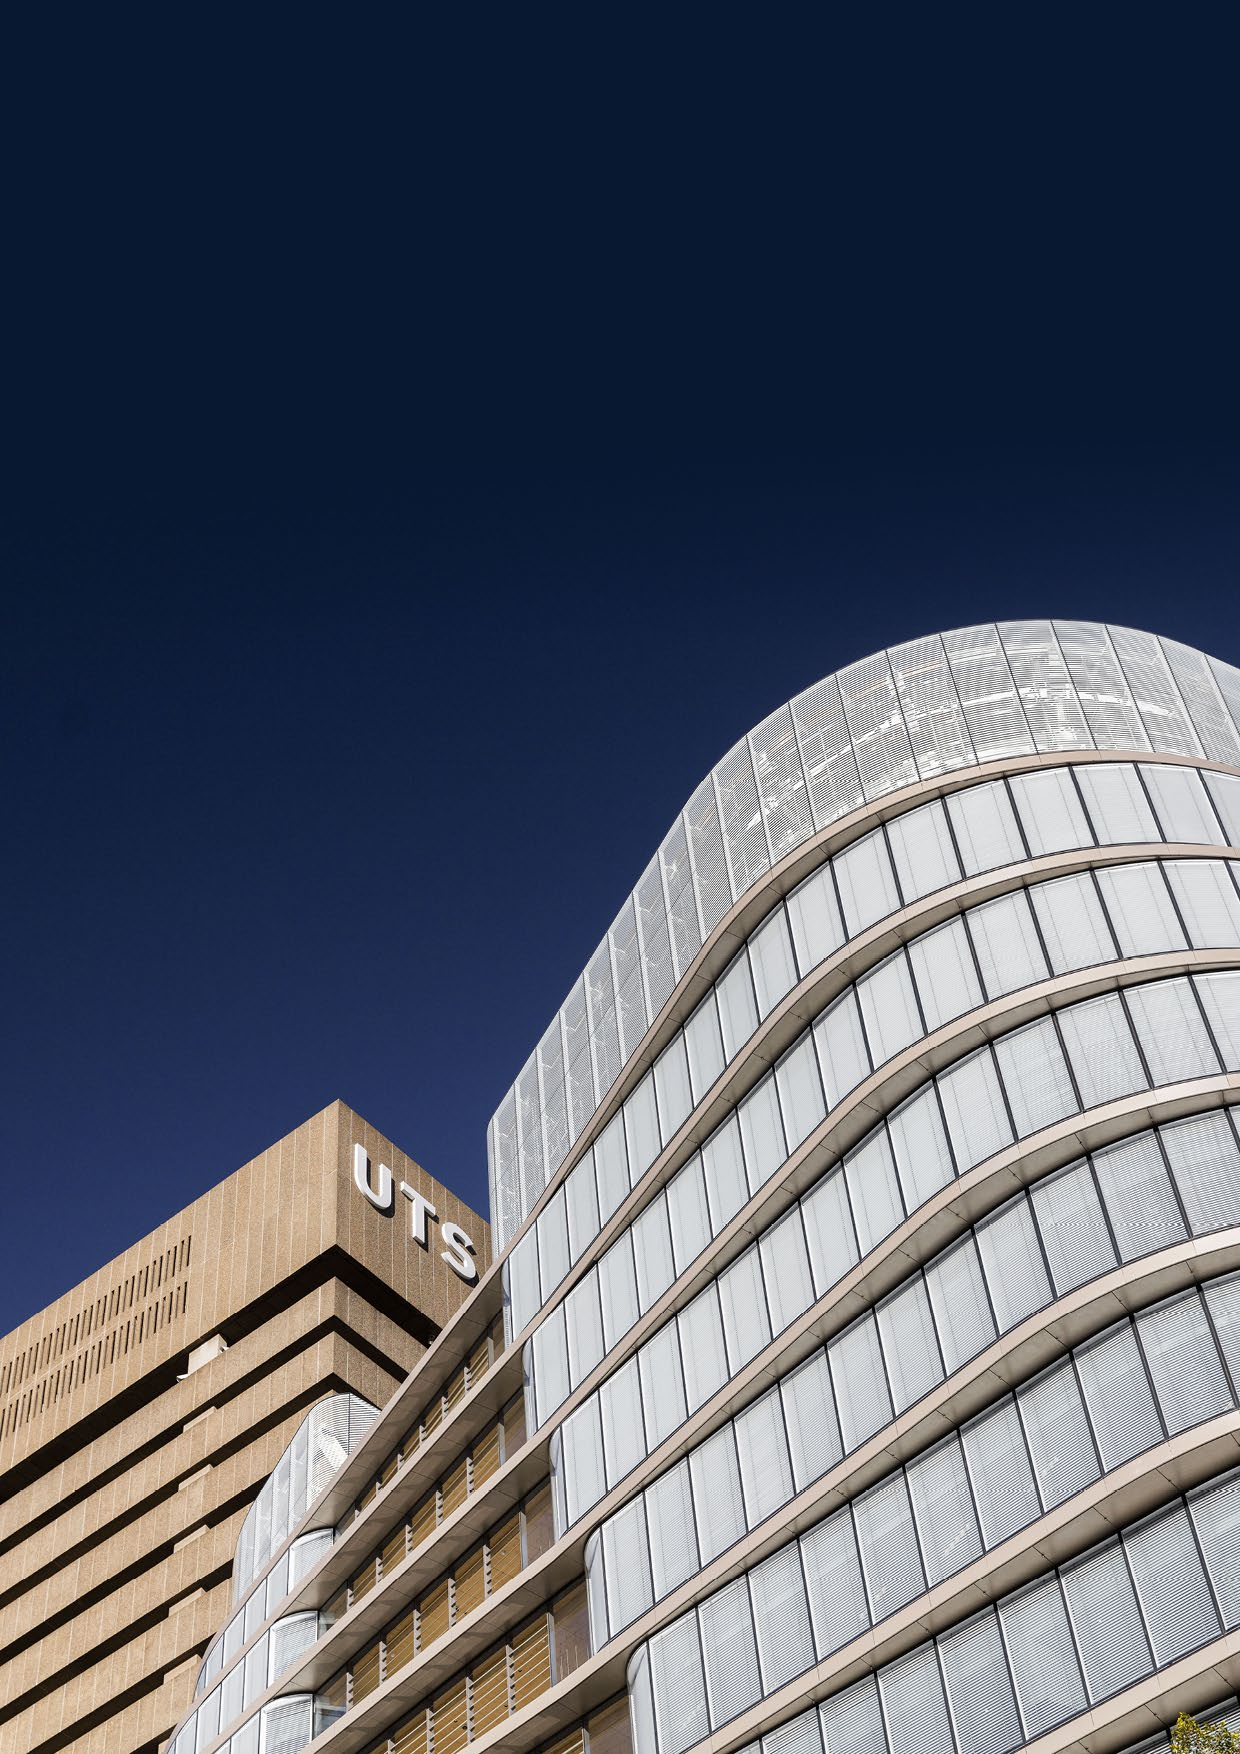
\includegraphics[width=\paperwidth]{img/The-Purpose-of-Public-Pol-002.jpg}}

\begin{tikzpicture}[remember picture, overlay]

\node[anchor=north east, xshift=-1.5cm, yshift=-1.5cm] at (current page.north east) {
    
\includegraphics[width=4.5cm]{img/uts_logo_white.png}
};

\node[
    anchor=north west,
    align=left,
    text width=0.7\paperwidth,
    xshift=1.5cm,
    yshift=-2.8cm 
] at (current page.north west) {
    \color{white}
    {\fontsize{32}{38}\selectfont\bfseries Assignment 2:}\\[0.3cm]
    {\fontsize{28}{34}\selectfont Data Analysis Report}
};

\node[
    anchor=north west,
    align=left,
    text width=0.7\paperwidth,
    xshift=1.5cm,
    yshift=-6cm
] at (current page.north west) {
    \color{white}
    {\rule{2cm}{1pt}}\\[0.4cm]
    {\fontsize{14}{18}\selectfont 36103: Statistical Thinking for Data Science}
};

\node[
    anchor=north west,
    align=left,
    text width=0.7\paperwidth,
    xshift=1.5cm,
    yshift=-7.3cm
] at (current page.north west) {
    \color{white}
    {\fontsize{10}{18}\selectfont \textbf{Submitted:} \today}
};

\node[
    anchor=south east,    
    align=left,
    fill=white,
    fill opacity=0.85, 
    text opacity=1,
    inner sep=20pt,
    rounded corners=1pt, 
    xshift=-1.5cm,          
    yshift=1.5cm          
] at (current page.south east) {
    \color{black}
    {\fontsize{12}{14}\selectfont \textbf{Group Number: 5}} \\[0.4cm]
    {\fontsize{10}{14}\selectfont
    \begin{tabular}{@{}l r@{}} 
    \textbf{Yash Bankar} & (25717428) \\
    \textbf{Preran Apinakoppa} & (26583524) \\
    \textbf{Bhavya Subhash Chandar} & (25599679) \\
    \textbf{Rohit Khanna} & (25669108) \\
    \textbf{Murphy Fang} & (26211831)
    \end{tabular}
    }
};

\end{tikzpicture}
\end{titlepage}


\pagenumbering{roman}

\vspace*{2.6cm}

{\begin{adjustwidth}{1.2cm}{1.2cm}
\setlength{\parindent}{0pt}
\section*{\LARGE Executive Summary}
\vspace*{1cm}
Electricity demand in NSW varies with weather, time, and season. During peak periods, wholesale prices can reach \$17,500/MWh, making accurate forecasts important for grid stability and cost management.

This project analysed NSW electricity data from 2022 to 2026 to identify demand patterns and develop forecasting models. Demand was lowest in mild weather, increased during extreme temperatures, and differed between weekdays and weekends. Rooftop solar reduced midday demand but increased evening peaks.

CatBoost was the best model, with an average error of about 389 MW. Its forecasts are useful for supporting operational decisions, especially under normal conditions.
\end{adjustwidth}}

\definecolor{bubble1}{HTML}{119dff}
\definecolor{bubble2}{HTML}{5b4fff}

\bubble[color=bubble1, opacity=1, x=-3.8, y=-5.6, size=8cm]{CatBoost achieved the best test performance: MAPE 4.45\%, Adjusted R² 0.884, MAE 389 MW. \\[0.3cm] XGBoost followed closely at 5.16\% and 0.860. Ridge Regression (10.3\%, 0.375) was insufficient for grid operations.}

\bubble[color=bubble2, opacity=1, x=3.8, y=-8, size=6.4cm]{Temperature and hour of day ranked as top predictors in both ensemble models, matching the U-shaped demand curve and intraday peaks from EDA.}

\clearpage

\tableofcontents

\clearpage
\listoftables
\listoffigures
\clearpage

\pagenumbering{arabic}

\sectionpage{Introduction}
\subsection{Problem Statement}
Electricity supply and demand must balance every 30 minutes. When they don't, grid operators absorb the cost. NSW wholesale prices can reach \$17,500/MWh under the market cap that applied through mid-2025 \citep{AER2025StateEnergyMarket}. Accurate short-term demand forecasting keeps dispatch decisions ahead of those spikes.  

\subsection{Rationale}
Serving 11 million customers, the NEM relies on NSW as its primary generator \citep{aer_our_role}. However, the lack of storage makes the grid vulnerable to demand swings. NSW’s 7.5 GW of rooftop solar (the highest globally per capita) creates a "duck curve" effect: suppressing midday demand before requiring a massive evening ramp from dispatchable generators \citep{cec_rooftop_solar_2025, green_solar_stats_2026}. This volatility drove 2024 wholesale prices up 43\% to \$150/MWh \citep{aer_wholesale_q4_2024}, making accurate forecasting critical to reducing costs. 
\subsection{Project Aims and Objectives}
The aim of this project was to determine whether machine learning models trained on historical half-hourly NSW data can predict grid electricity demand accurately enough to support operational dispatch planning. To support this aim, we asked: 


\begin{enumerate}[label=\textbf{\arabic*.}]
    \item Does temperature have a non-linear relationship with NSW grid demand across 2\textdegree{}C bins from 5\textdegree{}C to 43\textdegree{}C?
    \item Do mean hourly demand profiles differ between weekdays, weekends, and public holidays in NSW?
    \item Can an ensemble regression model predict 30-minute NSW grid demand with a MAPE below 5\% on held-out test data? 
\end{enumerate}

To answer these questions, we sourced and merged half-hourly AEMO data with weather, rooftop solar, and economic indicators, then ran exploratory analysis to identify key demand drivers. We built and compared Ridge Regression, XGBoost, and CatBoost models on a 60:20:20 chronological split, evaluating each on RMSE, MAE, MAPE, and Adjusted R². 

\sectionpage{Methodology}
\subsection{Dataset}
\subsubsection{Data Acquisition and Cleaning}
While raw AEMO market data was high-frequency, it lacked the exogenous environmental and economic features crucial for predictive modelling. Time-stamps were utilised as the primary keys to synthetically merge weather and economic datasets into a unified feature set. Cleaning involved linear interpolation of missing observations, removing high multi-collinear features and frequency alignments. Please refer to \appcref{app:eda} for a comprehensive \textbf{EDA}.


\begin{table}[H]
    \centering
    \caption{Data Collation and Source Rationale}
    \label{tab:data_sources}
    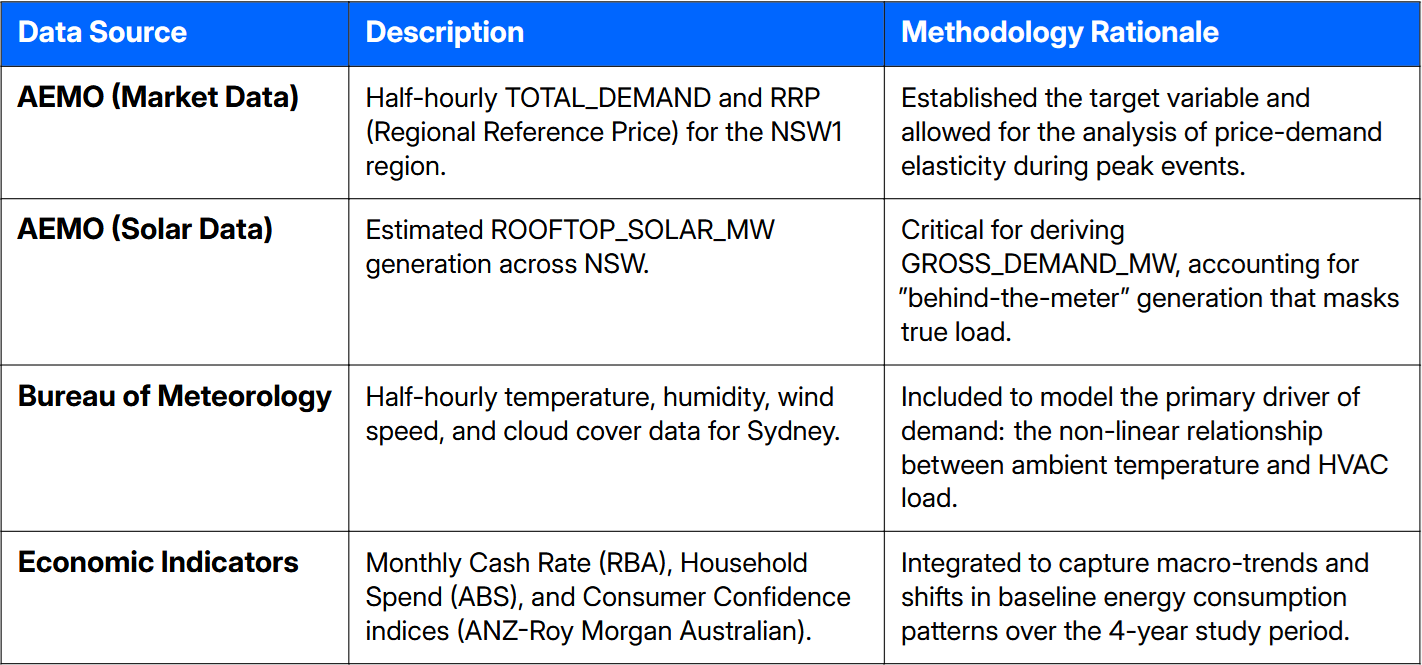
\includegraphics[width=0.8\textwidth]{img/table1.png}
\end{table}

\subsubsection{Feature Scaling}
For better generalisation and to remove individuality in entries, the following feature scaling processes were completed:

\begin{itemize}
  \item \textbf{Feature Engineering:} The hour, minute, weekend and month were extracted from the \texttt{DATE\_TIME} feature.
  \item \textbf{Data Transformation:} One-Hot Encoding (OHE) was applied to categorical columns, standard scaling for numerical columns and binary 0/1 for boolean features. 
\end{itemize}

\subsection{Technologies Used}
Developed in a Python 3.11 virtual environment, BeautifulSoup for web scraping, Pandas for data-frames, CatBoost and XGBoost libraries, scikit-learn, and Vegas-Altair for visualisation. Seeding was set to 42 for consistency and reproducibility. Resulted in 70,176 rows across 28 features. Chronologically split in 60:20:20 provided 42105:14035:14036 rows for training, validation and testing respectively.

\begin{figure}[H]
  \centering
  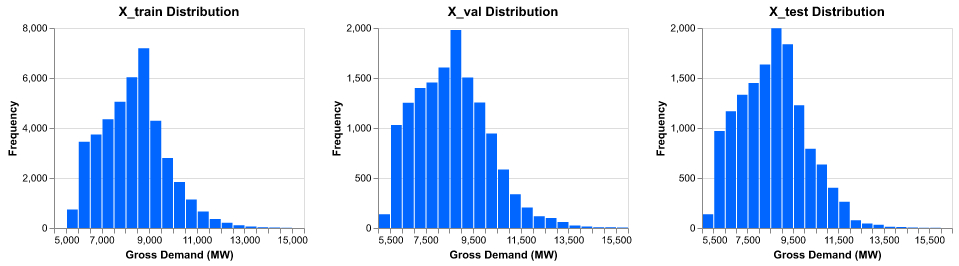
\includegraphics[width=\textwidth]{img/dist_chart.png}
  \caption{Target feature distribution}
\end{figure}

\subsection{Models}
\subsubsection{Linear Regression (Ridge)}
The linear regressor is a parametric model that fits a linear equation over observational data. A Ridge variant served as the baseline for its computational efficiency, stability via L2 regularisation, and ability to mitigate multicollinearity among correlated weather features.

\subsubsection{Gradient Boosting Decision Trees}
Gradient Boosted Decision Trees (GBDT) are a non-parametric ensemble models that sequentially build decision trees, using gradient descent to minimise the residual loss of the previous ensemble.

\begin{table}[H]
    \centering
    \caption{Model Selection and Theoretical Rationale}
    \label{tab:models}
    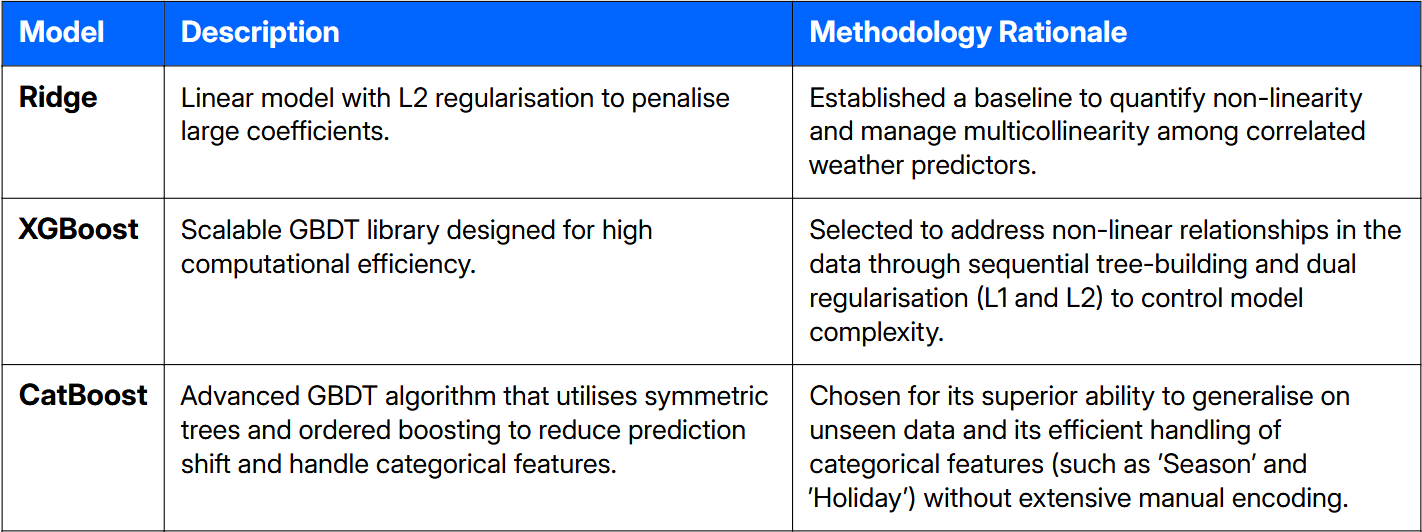
\includegraphics[width=0.8\textwidth]{img/table2.png}
\end{table}

\subsection{Grid Search}
Hyperparameter optimisation is performed via Grid Search with \(k\)-fold Cross-Validation. Through exhaustive predefined parameter grids, we identified configurations that minimised generalisation error of each model.

\subsection{Metrics}

\begin{table}[h]
  \centering
  \caption{Chosen Performance Metrics}
  \label{tab:metrics_desc}
  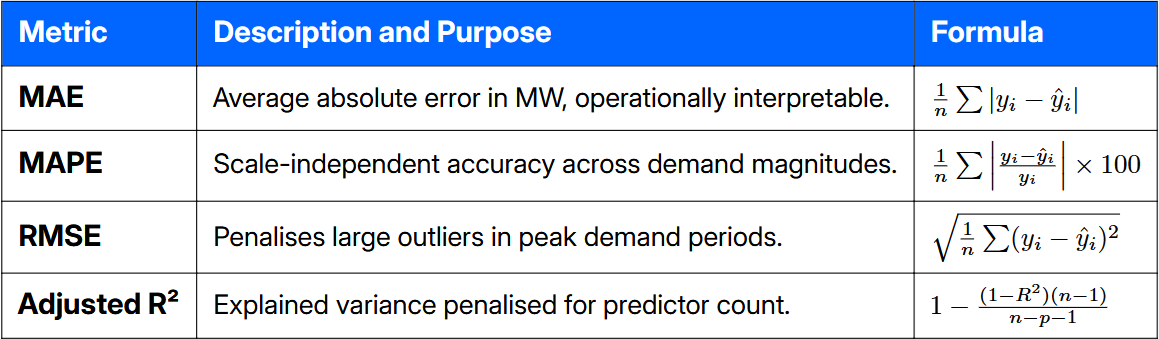
\includegraphics[width=0.6\textwidth]{img/table3.png}
  \end{table}
  
Model performance was evaluated using a hold-out test set to ensure generalisability. The following \autoref{tab:metrics_desc} above illustrates the chosen metrics.


\sectionpage{Results}
\subsection{Key Findings}
CatBoost achieved the best test performance (MAPE 4.47\%, Adj. R² = 0.872, MAE = 400.25 MW), meeting the sub-5\% accuracy target. Surprisingly, Ridge Regression explained only 38.9\% of demand variation despite regularisation, confirming NSW electricity demand is fundamentally non-linear.

\subsection{In-depth Results}

\subsubsection{Can an ensemble regression model predict 30-minute NSW grid demand with MAPE below 5\%?}

\begin{table}[h]
\centering
\caption{Model Performance Comparison}
\label{tab:model_performance}
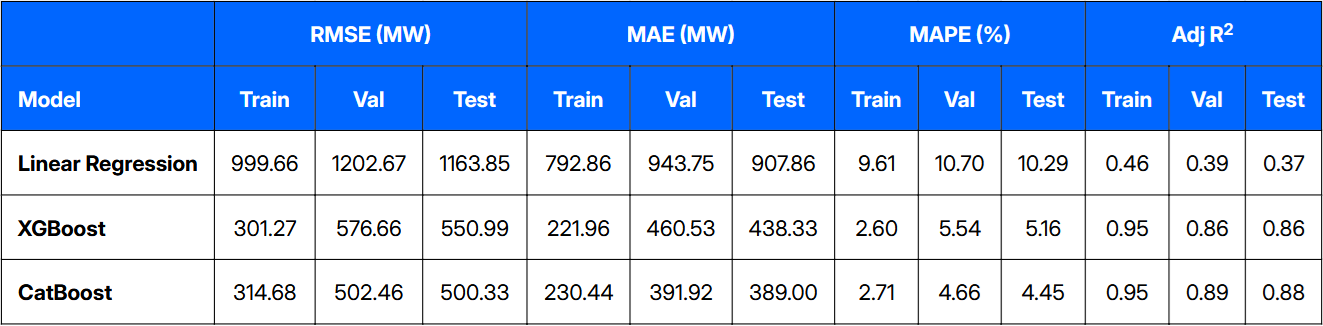
\includegraphics[width=0.8\textwidth]{img/table4.png}
\end{table}

Three models were compared on held-out test data (\autoref{tab:model_performance}). Ridge Regression failed to capture non-linear patterns (MAPE 10.31\%, R² = 0.389). XGBoost improved but showed overfitting (MAPE 5.83\%, R² = 0.836). CatBoost generalised best across all metrics, meeting the sub-5\% threshold.

\begin{figure}[H]
  \centering
  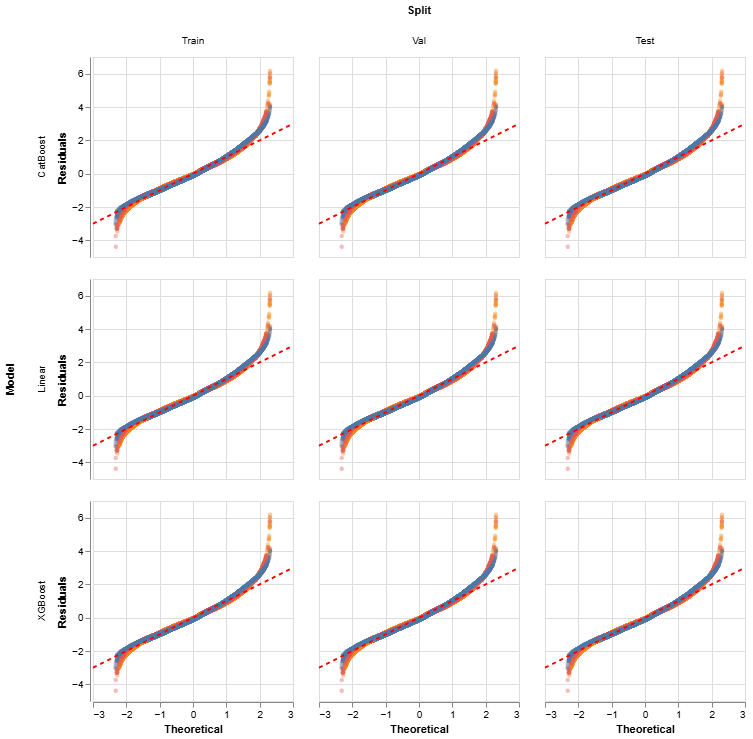
\includegraphics[width=0.7\textwidth]{img/qqplots.png}
  \caption{QQ-plots. All models show reasonable normality in the central quantile range with heavier tails at extremes, consistent with demand spikes during extreme weather events.}
  \label{fig:qq_plots}
\end{figure}

Regression assumptions were verified via QQ-plots (shown in \autoref{fig:qq_plots}).

\subsubsection{Model Interpretation and Feature Importance}
Feature importance comparisons (\autoref{fig:feature_comparison}) indicate that while the Ridge baseline relied on temperature, CatBoost and XGBoost prioritised temporal and environmental drivers. This confirms the boosted models learned solar patterns through proxies, successfully compensating for the removed rooftop solar feature.

\begin{figure}[H]
     \centering
     \begin{subfigure}[b]{0.48\textwidth}
         \centering
         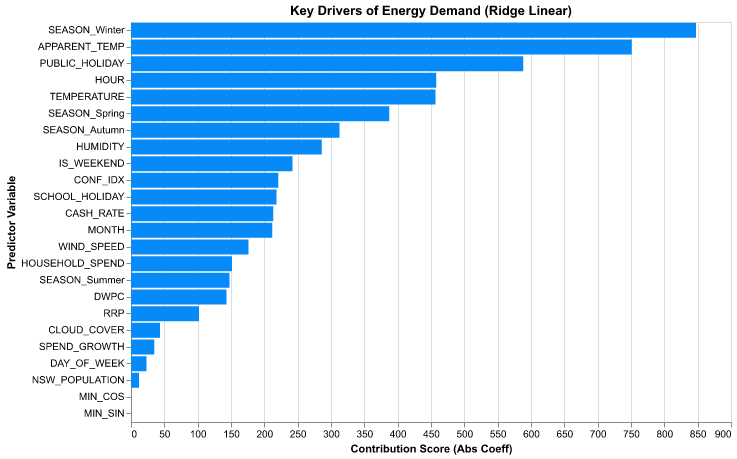
\includegraphics[width=\textwidth]{img/lin_imp_chart.png}
         \caption{Ridge (Baseline)}
         \label{fig:imp_ridge}
     \end{subfigure}
     \hfill
     \begin{subfigure}[b]{0.48\textwidth}
         \centering
         
\includegraphics[width=\textwidth]{img/xgb_imp_chart.png}
         \caption{XGBoost}
         \label{fig:imp_xgb}
     \end{subfigure}
     \hfill
     \begin{subfigure}[b]{0.48\textwidth}
         \centering
         
\includegraphics[width=\textwidth]{img/cat_imp_chart.png}
         \caption{CatBoost}
         \label{fig:imp_cat}
     \end{subfigure}
        \caption{Feature Importance Comparison across Models}
        \label{fig:feature_comparison}
\end{figure}

Conversely, the marginal impact of the \textbf{Cash Rate} suggest that while economic indicators provide macro-context, they are less critical for short-term 30-minute interval forecasting than environmental and temporal features.

\sectionpage{Conclusion}
\subsection{Conclusion}
CatBoost forecasts NSW grid demand to within 4.47\% average error; useful for dispatch planning, but not a replacement for operator judgement during extreme or unusual conditions.
\subsection{Discussion}
This project evaluated machine learning for grid dispatch using historical NSW half-hourly data. \textbf{CatBoost} met the sub-5\% target, achieving a \textbf{4.47\% MAPE} and \textbf{0.872 $R^2$} ($\approx$400~MW MAE). Conversely, \textbf{XGBoost} overfit, while \textbf{Ridge Regression} failed (10.31\% MAPE), confirming NSW demand is non-linear. At average 2024 prices (\$150/MWh), a 400~MW error represents a significant financial risk.

\subsection{Project Limitations and Caveats}
The model is fixed to a 2022-2026 training window with no self-update mechanism. Accuracy will drift as the grid changes. Urban areas also dominate the dataset, so regional and remote NSW performance is likely worse than the headline numbers suggest.

Remote and Aboriginal communities are underrepresented in AEMO grid data. A model trained mainly on urban demand risks reinforcing unequal energy distribution if applied broadly. Any deployment should respect Indigenous Data Sovereignty principles and involve community engagement before rollout.

\subsection{Stakeholder Analysis and Project Outcomes}
The deliverable is a CatBoost pipeline returning 30-minute demand forecasts from weather, calendar, and economic inputs. AEMO operators benefit most, in that the better forecasts mean less reliance on expensive last-minute generation. Next steps: live AEMO data integration, retraining cadence, and testing sequential models like LSTM for extreme weather periods.

\clearpage
%TC:ignore
\sectionpageunum{References}
\printbibliography[heading=none]
\clearpage
\begin{appendices}
\sectionpageunum{Appendices}
\section{Exploratory Data Analysis}
\label[appendix]{app:eda}
The objective of this exploratory phase was to move beyond the raw complexity to identify the primary drivers of Gross Energy Demand. In light of the data science project cycle, this EDA served two critical functions: \textbf{Feature Selection} and \textbf{Operational Insights}.

\subsection{General Exploration}
Observing multicollinearity such as through a correlation heatmap is critical because it identifies highly redundant predictors that can destabilise the model, inflate the variance of coefficient estimates, and make it impossible to determine the individual mathematical contribution of each variable to the target output.
\begin{figure}[H]
    \centering
    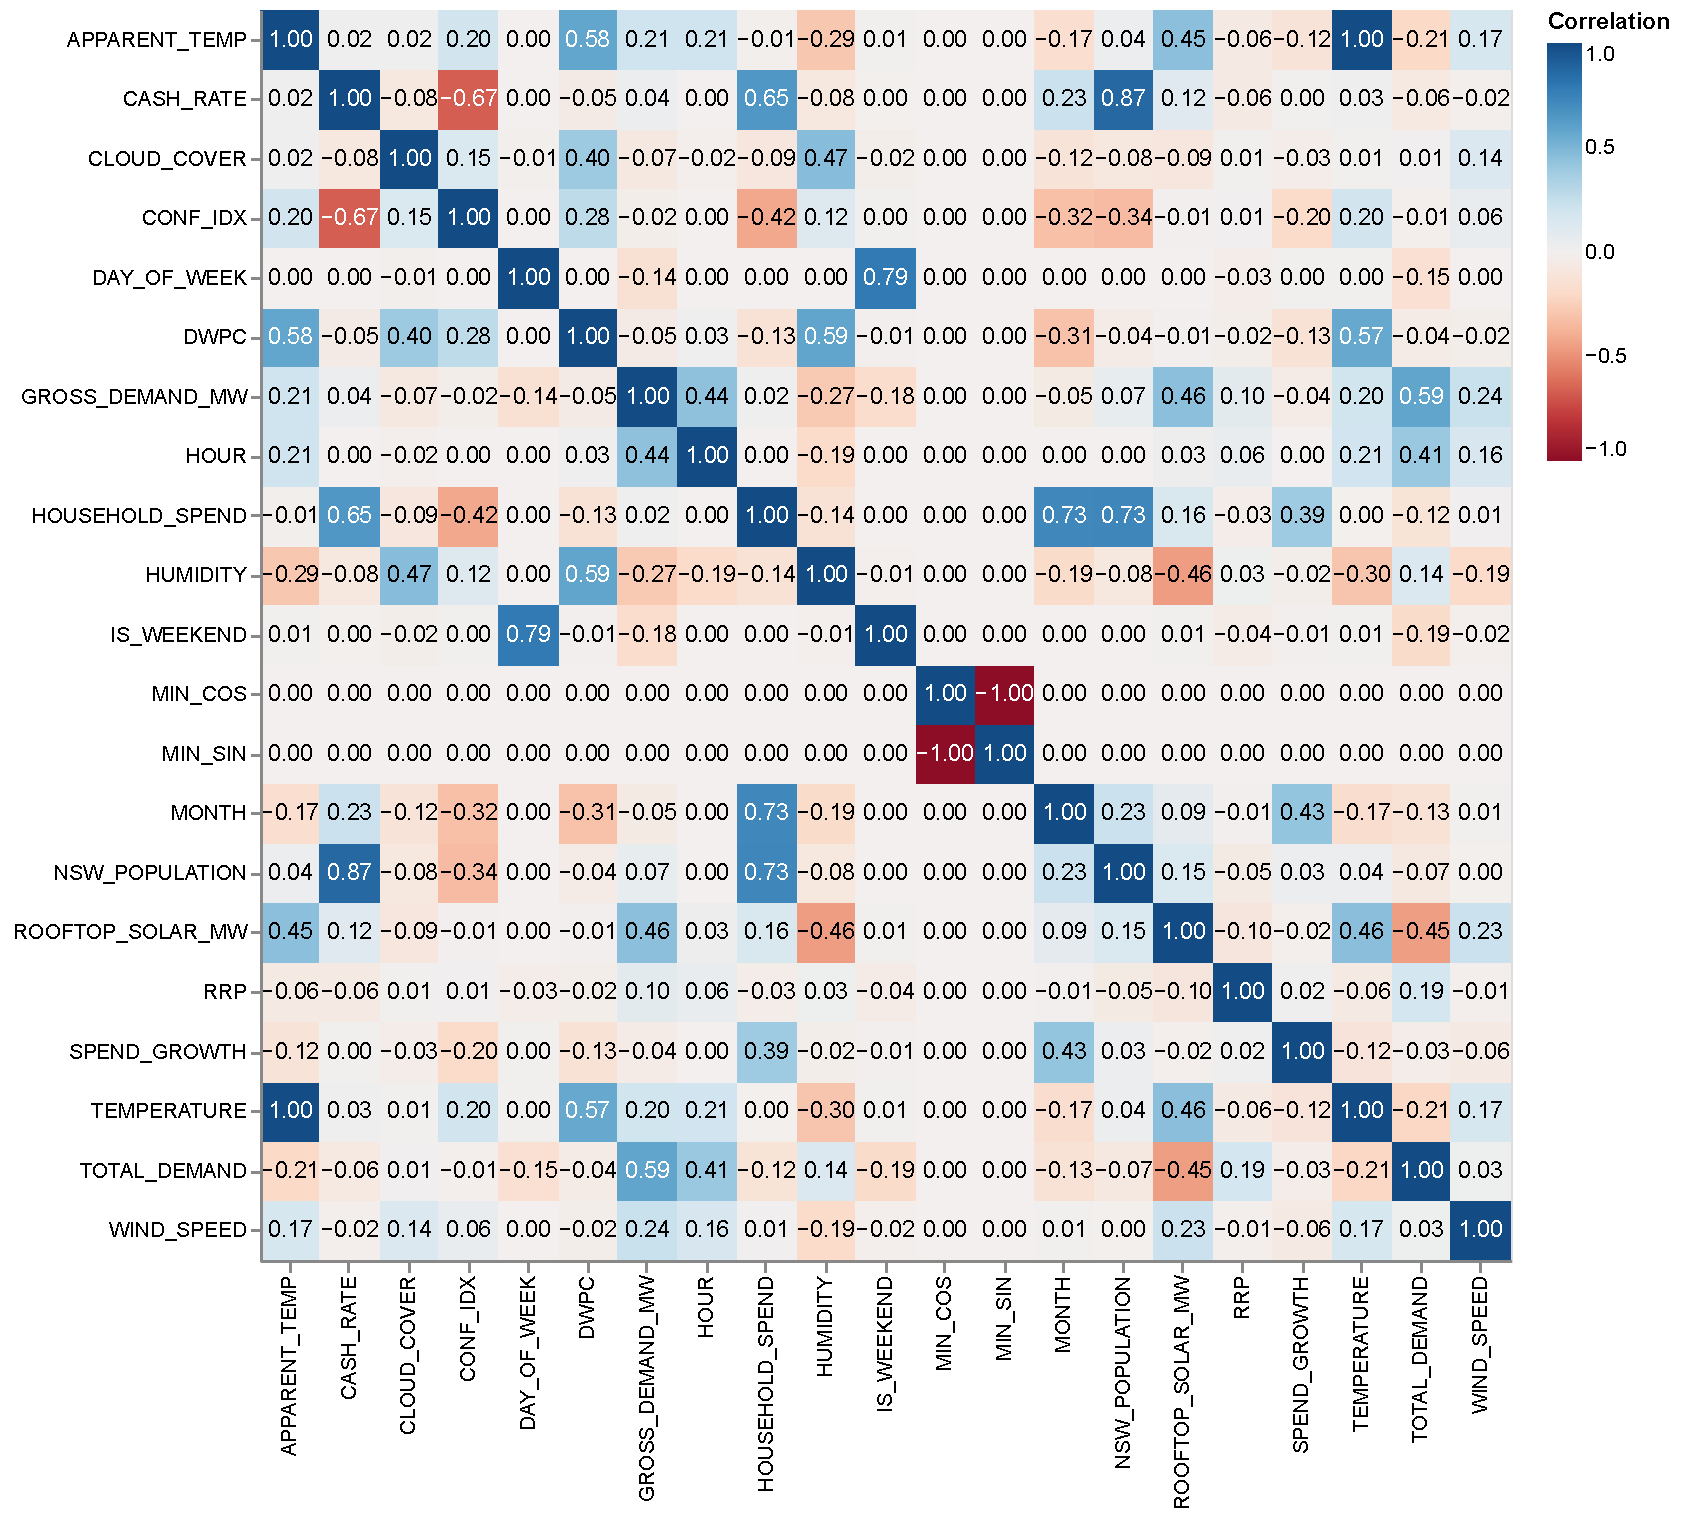
\includegraphics[width=\linewidth]{img/multicollinearity_chart.pdf}
    \caption{Multicollinearity Matrix on Raw Data}
\end{figure}

\subsection{Does temperature have a non-linear relationship with NSW grid demand across 2°C bins?}
A clear U-shaped relationship was observed between temperature and mean grid demand (\autoref{fig:rq1}). Demand was lowest near 21°C and rose sharply at both cold and hot extremes, directly ruling out linear modelling.

\begin{figure}[H]
  \centering
  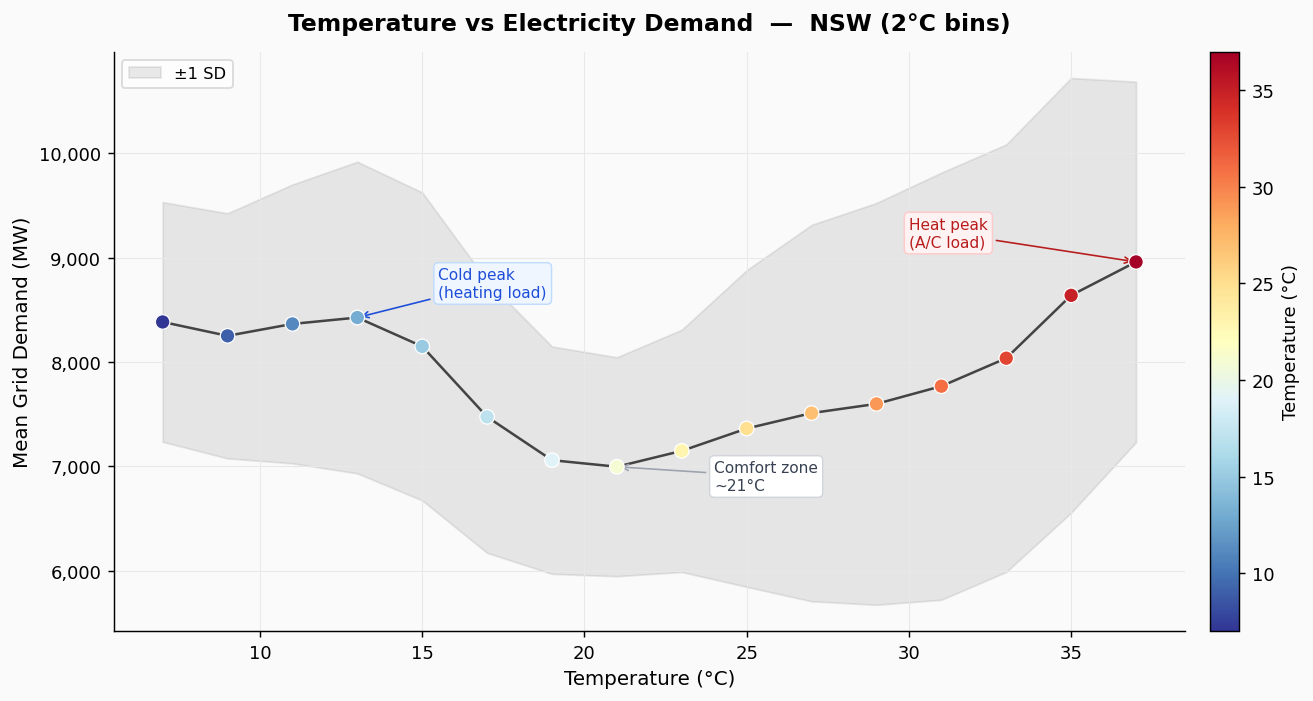
\includegraphics[width=0.8\textwidth]{img/rq1_temp_vs_demand.png}
  \caption[Mean NSW grid electricity demand across temperature bins.]{Mean NSW grid electricity demand (MW) across 2°C temperature bins (5°C-43°C). A U-shaped pattern is evident, with lowest demand near the comfort zone ($\sim$21°C, $\sim$7,000 MW), rising at cold extremes due to heating load and hot extremes due to air-conditioning. Shaded band represents ±1 SD.}
  \label{fig:rq1}
\end{figure}


\subsection{Do mean hourly demand profiles differ between weekdays, weekends, and public holidays?}
Weekday demand showed a morning commercial peak at 8 AM ($\sim$8,200 MW) and an evening residential peak at 7 PM ($\sim$9,500 MW). Weekend and holiday profiles were 1,000-1,500 MW lower with no morning peak (\autoref{fig:rq2}). An unexpected finding was a pronounced midday dip across all day types driven by rooftop solar, forming the classic “duck curve” pattern (\autoref{fig:rq3}).

\begin{figure}[H]
  \centering
  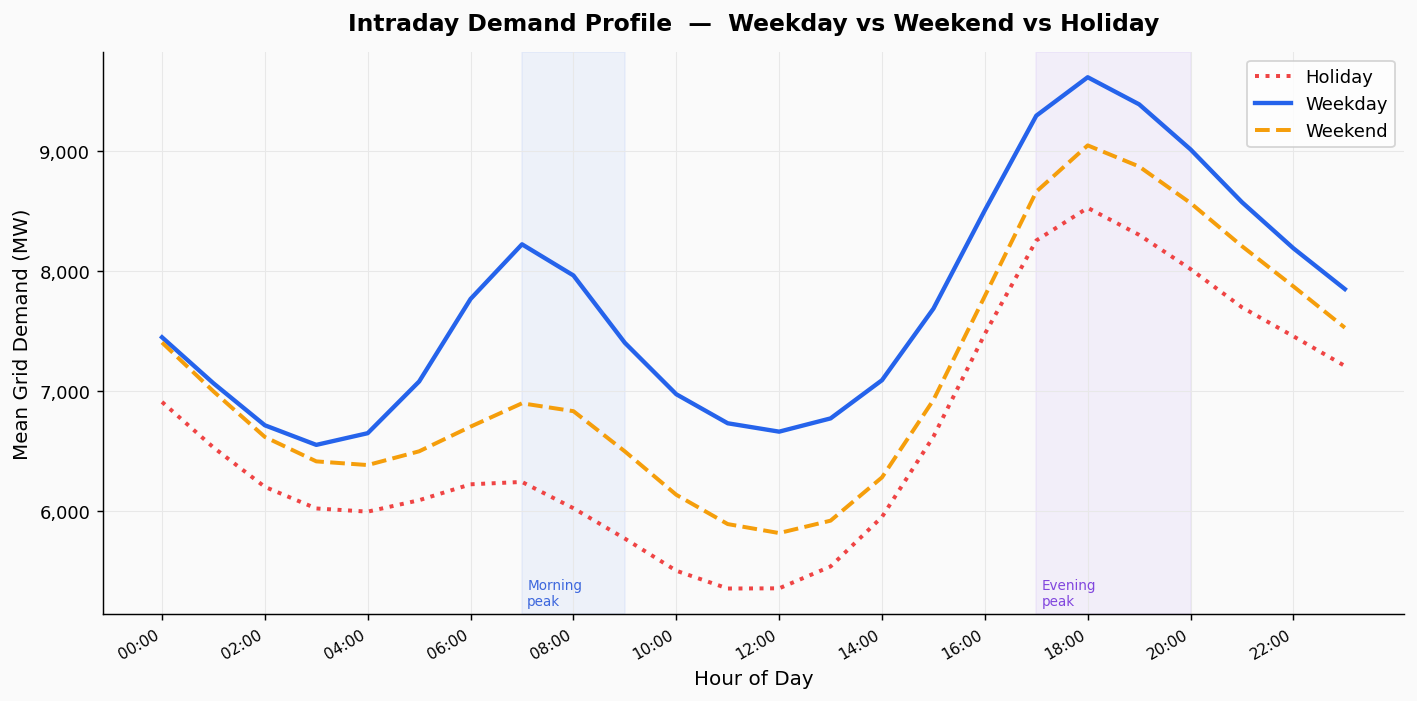
\includegraphics[width=0.8\textwidth]{img/rq2_intraday_demand.png}
  \caption[Mean NSW intraday electricity demand by day type.]{Mean NSW grid electricity demand (MW) by hour of day for weekdays (solid blue), weekends (dashed orange), and public holidays (dotted red). Weekdays show a morning peak at 8 AM ($\sim$8,200 MW) and an evening peak at 7 PM ($\sim$9,500 MW). Weekend and holiday profiles are 1,000-1,500 MW lower with no commercial morning peak.}
  \label{fig:rq2}
\end{figure}

\begin{figure}[H]
  \centering
  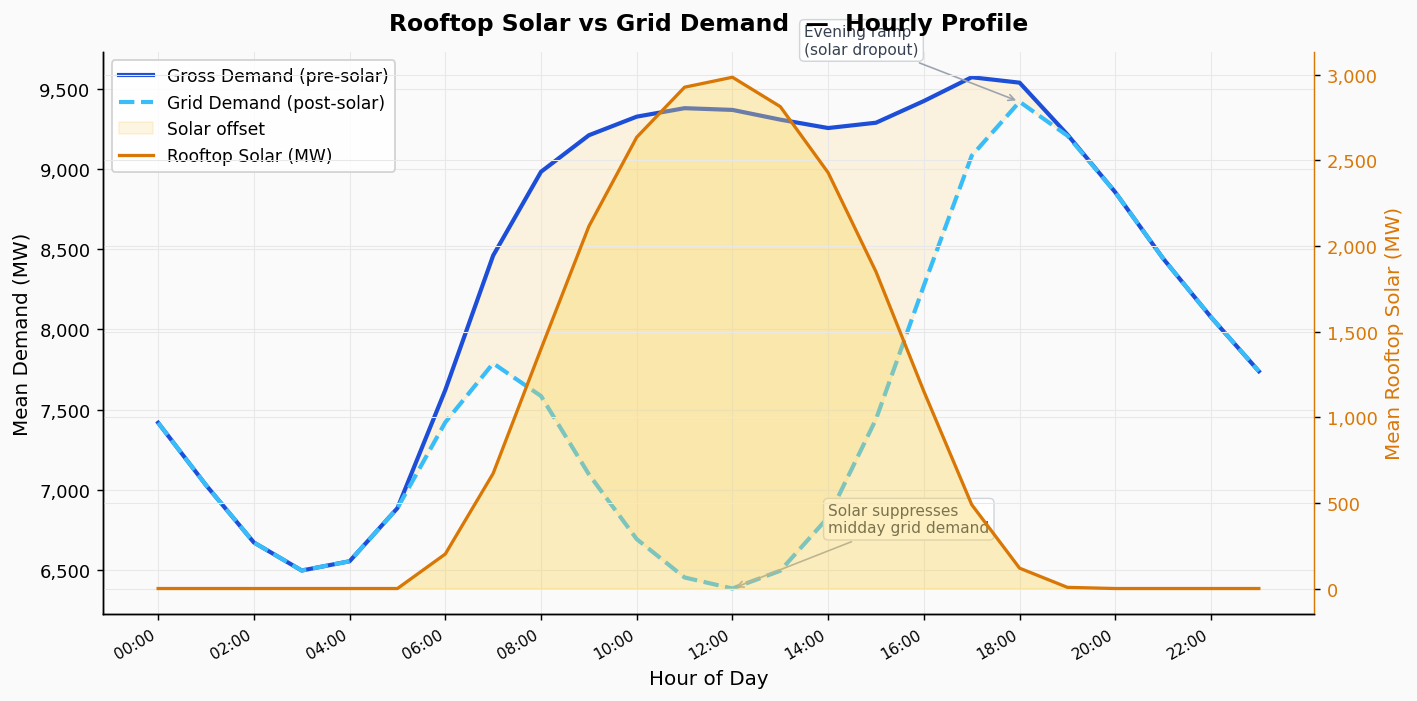
\includegraphics[width=0.8\textwidth]{img/rq3_solar_vs_demand.png}
  \caption[Impact of rooftop solar on NSW grid demand (the "duck curve").]{Mean hourly rooftop solar generation (MW, right axis, orange) overlaid on gross pre-solar demand (solid blue) and net post-solar grid demand (dashed teal). Solar peaks near midday ($\sim$3,000 MW), suppressing grid demand and creating the sharp evening ramp as generation drops — the “duck curve” pattern.}
  \label{fig:rq3}
\end{figure}
\clearpage
\section{Modelling Code}
\subsection{Data Preparation}
\lstinputlisting[language=Python]{scripts/preparation.py}

\subsection{Modelling}
\lstinputlisting[language=Python]{scripts/modelling.py}
%TC:endignore
\end{appendices}
\end{document}